\cleardoublepage

\chapter{Retrieval Augmented Generation (RAGs)}
\label{Retrieval Augmented Generation (RAGs)}

Para este capítulo se ha usado el artículo \textit{Retrieval-augmented generation for large language models: A survey} \citep{gao2023retrieval}

\section{Introducción}

El \textit{Retrieval-Augmented Generation} (RAG) ha emergido como una solución efectiva para superar algunas de las limitaciones de los LLMs, como las alucinaciones y la incapacidad de manejar información actualizada o específica de un dominio. RAG integra la generación de respuestas de los LLMs con la recuperación de información de bases de datos externas, permitiendo que los modelos de lenguaje accedan a información más precisa y reciente.

\section{Motivación y Aplicaciones}

Los LLMs son conocidos por generar contenido no siempre veraz, especialmente cuando se enfrentan a preguntas fuera de su conjunto de datos de entrenamiento. Aquí es donde el RAG entra en juego: este método permite a los LLMs consultar bases de datos externas para recuperar documentos relevantes y aumentar su conocimiento con información específica y precisa. Esta combinación ha demostrado ser particularmente útil en tareas intensivas en conocimiento, como la resolución de preguntas complejas y en la integración de datos especializados.


\section{Componentes Principales}

El marco de RAG se compone principalmente de tres etapas: recuperación, generación y aumento (retrieval, generation y augmentation, respectivamente). Cada una de estas etapas desempeña un papel fundamental en la mejora del rendimiento del LLM:

\begin{itemize}
    \item \textbf{Recuperación}: Esta etapa implica la búsqueda de fragmentos de documentos relevantes a partir de bases de datos externas, utilizando medidas de similitud semántica. Esto asegura que la generación de texto se base en información actual y precisa.
    \item \textbf{Generación}: Una vez recuperados los fragmentos, el modelo genera respuestas utilizando tanto la consulta inicial como la información recuperada. Este proceso ayuda a evitar la generación de contenido incorrecto o alucinado.
    \item \textbf{Aumento}: Finalmente, el proceso de aumento integra la información recuperada con el contexto de la tarea, mejorando así la calidad y relevancia de la salida del modelo.
\end{itemize}

Una ilustración visual del flujo de trabajo en un sistema RAG se muestra en la Figura \ref{fig:rag}. En esta imagen, se puede observar cómo el usuario realiza una consulta inicial y, se muestra como el LLM podría responder directamente a la pregunta de manera descontextualizada o cómo puede mediante el uso de un RAG contextualizar la pregunta. Para ello, como primer paso los documentos son fragmentados y convertidos en vectores para su comparación semántica. Luego, el LLM utiliza estos fragmentos recuperados para generar una respuesta más precisa y contextualizada.

\begin{figure}[h]
    \centering
    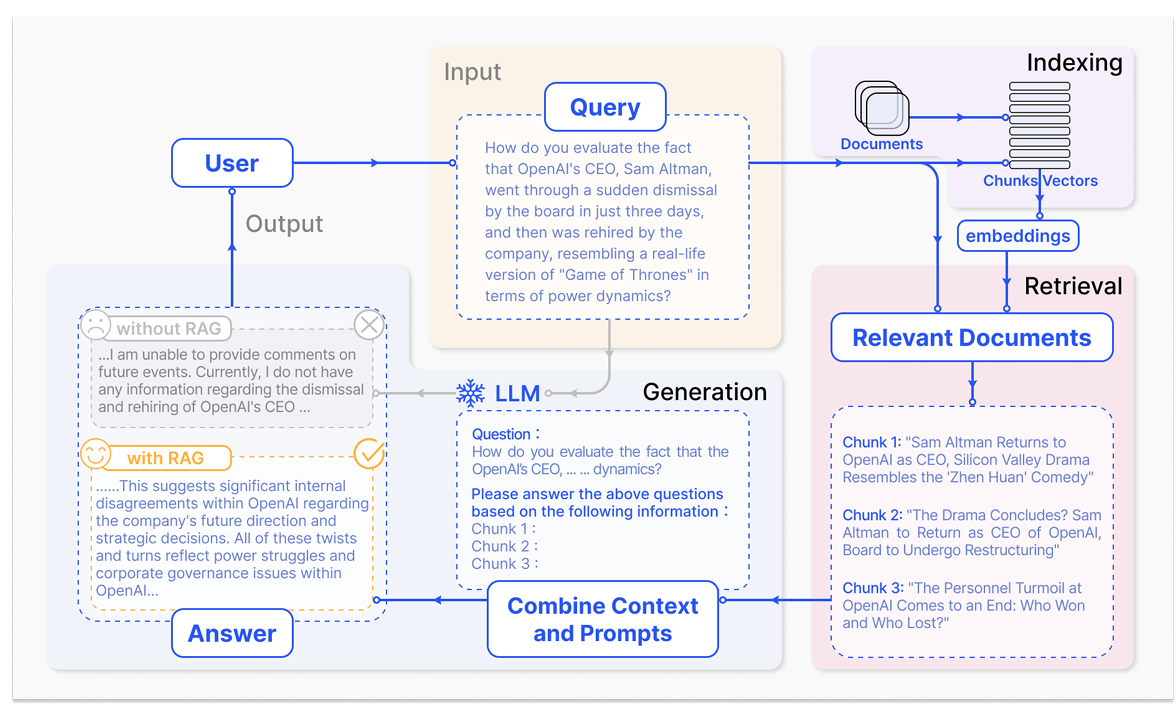
\includegraphics[width=0.8\textwidth]{figuras/capitulo2/rag.png}
    \caption{Flujo de trabajo de RAG mostrando la integración de documentos recuperados para mejorar la generación de texto.}
    \label{fig:rag}
\end{figure}

Como se muestra en la Figura \ref{fig:rag}, el uso de RAG mejora significativamente la calidad de las respuestas generadas por el LLM al proporcionar información adicional relevante. Sin RAG, el modelo puede verse limitado a sus conocimientos previos y no ser capaz de manejar eventos recientes o información específica. Con RAG, el modelo puede acceder a documentos actualizados que enriquecen sus respuestas, como es el caso del ejemplo de la figura en donde el LLM es capaz de dar un análisis detallado del despido y la recontratación del CEO de OpenAI, basado en noticias recuperadas. 

\subsection{Embeddings en Retrieval-Augmented Generation}

En el contexto de Retrieval-Augmented Generation (RAG), los \textit{embeddings} juegan un papel crucial para conectar de manera efectiva los sistemas de recuperación y generación de texto. Un \textit{embedding} es una representación numérica de un fragmento de texto, que captura su significado semántico en un espacio de alta dimensión, permitiendo que los algoritmos de recuperación encuentren información relevante mediante la comparación de similitudes semánticas en lugar de simples coincidencias de palabras clave \cite{cloudgirl2023rag, datastax2023rag}.

\textbf{Proceso de Vectorización}: El proceso de creación de \textit{embeddings} comienza dividiendo el texto en fragmentos manejables, a menudo denominados \textit{chunks}. Estos fragmentos son transformados en vectores utilizando modelos de aprendizaje automático especializados, como \textit{word2vec} o \textit{sentence transformers}. Estos modelos de \textit{embeddings} están diseñados para representar el contexto y el significado de los fragmentos de texto de manera que los vectores de fragmentos similares estén más cerca unos de otros en el espacio vectorial \cite{nvidia2023rag}.

Una vez creados, estos vectores se almacenan en bases de datos vectoriales especializadas, como Pinecone, Milvus o Faiss, que están optimizadas para la recuperación rápida de información basada en similitudes vectoriales. Esto permite que el sistema de recuperación encuentre rápidamente fragmentos de texto que sean relevantes para una consulta dada \cite{datastax2023rag}.

\textbf{Función en RAG}: Los \textit{embeddings} son esenciales para el funcionamiento del sistema RAG. Cuando se presenta una consulta, el sistema genera un \textit{embedding} para dicha consulta y lo compara con los \textit{embeddings} almacenados en la base de datos vectorial. Este proceso de búsqueda vectorial permite que el sistema identifique los fragmentos de texto más relevantes en función de su similitud semántica con la consulta \cite{cloudgirl2023rag}. Estos fragmentos recuperados luego se integran en la generación de respuestas del modelo de lenguaje, mejorando la precisión y relevancia de las respuestas al proporcionar información actualizada y específica del contexto.

\textbf{Almacenamiento y Procesamiento de los Embeddings}: Para maximizar la eficiencia, los \textit{embeddings} se almacenan en bases de datos vectoriales optimizadas para la búsqueda y recuperación de datos en espacios de alta dimensión. Esto permite que el sistema de RAG maneje grandes volúmenes de información de manera eficiente, ofreciendo respuestas precisas basadas en datos externos relevantes que enriquecen la salida generada por los LLMs \cite{nanonets2023rag}.

\begin{figure}[h]
    \centering
    \begin{subfigure}[b]{0.45\textwidth}
        \centering
        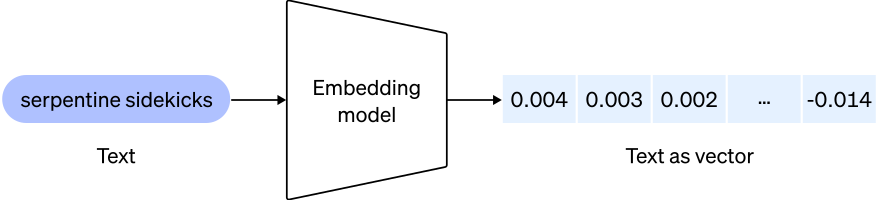
\includegraphics[width=\textwidth]{figuras/capitulo2/vectors-3.png}
        \label{fig:rag1}
    \end{subfigure}
    \hfill
    \begin{subfigure}[b]{0.45\textwidth}
        \centering
        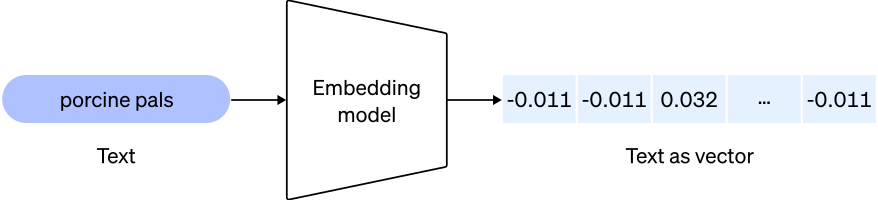
\includegraphics[width=\textwidth]{figuras/capitulo2/vectors-2.png}
        \label{fig:rag2}
    \end{subfigure}
    \caption{Ejemplos de embeddings. \citep{openai}}
    \label{fig:embeddigns}
\end{figure}


En resumen, los \textit{embeddings} son la columna vertebral del sistema de recuperación en RAG, permitiendo que los modelos de lenguaje accedan a información relevante de manera eficiente, lo que resulta en respuestas más precisas y contextualmente ricas \cite{cloudgirl2023rag, nvidia2023rag}.


\section{Desafíos y Futuras Direcciones}

A pesar de su éxito, el RAG enfrenta varios desafíos. Uno de los principales es la necesidad de manejar información ruidosa o contradictoria, lo que puede afectar la calidad de la generación de texto. Además, los desarrollos futuros buscan mejorar la integración de datos de múltiples fuentes y mejorar la capacidad de los modelos para adaptarse a tareas más complejas.

